\section{Comparación de preferencias}

\begin{frame}{Comparación de preferencias}
	\begin{description}
		\item[Entrada:] Vector de enteros \texttt{v} y su tamaño \texttt{n}
		\item[Salida:] Entero no negativo que indica el número de pares $i,j$ de posiciones del vector tales que $i < j$ y $v[i] > v[j]$
	\end{description}
\end{frame}

\subsection{Algoritmos}

\begin{frame}[fragile]{Algoritmo obvio}
	Recorre cada par de elementos $i,j : i < j$ y comprueba si $v[i] > v[j]$, sumando a un contador en tal caso:
	\lstinputlisting[firstline=24, lastline=32]{cpps/preferencias.cpp}
	\textbf{Eficiencia:} $O(n^2)$.
\end{frame}

\begin{frame}[fragile]{Algoritmo Divide y Vencerás}
	El número de inversiones es igual a la suma de:
	\begin{itemize}
		\item El número de pares invertidos en el subvector a la izquierda.
		\item El número de pares invertidos en el subvector a la derecha.
		\item El número de pares invertidos de subvectores distintos.
	\end{itemize}
	
	\pause
	Usando \textit{mergesort}, el tercer sumando se reduce a sumar cuántos elementos del primer subvector están pendientes de ser insertados en la mezcla cada vez que se inserta un elemento del segundo subvector.
	
	\pause
	
	Por debajo de un cierto umbral usaremos la ordenación por inserción, que también puede usarse para contar el número de inversiones.
	
	\textbf{Eficiencia:} $O(n \cdot \log(n))$.
	%No podemos usar el algoritmo obvio para esto porque, al mezclar, el \textit{mergesort} supone que los subvectores se encuentran ordenados, así que deben estar ordenados.
\end{frame}

% TODO: ¿Códigos? (son larguillos y divididos en trozos) ¿Presentar también inserción modificado? ¿Es necesario justificar que es O(n·log(n))?

\begin{frame}[fragile]{Ejemplo}
	\begin{center}
	\vspace{-0.4cm}
	\hspace{-2cm}
	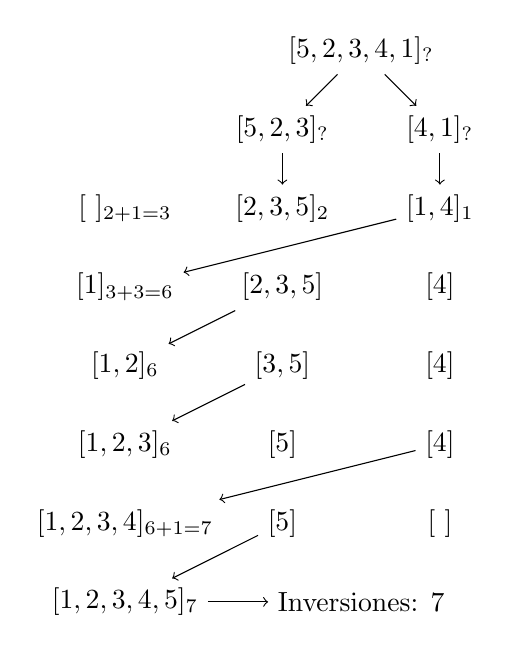
\begin{tikzpicture}
		\node (T0) at (0,0) {$[5,2,3,4,1]_?$};
		\pause
		\node (Uu) at (-1,-1) {$[5,2,3]_?$};
		\node (Vu) at (1,-1) {$[4,1]_?$};
		\draw [->] (T0) -- (Uu);
		\draw [->] (T0) -- (Vu);
		\pause
		\node (Uo) at (-1,-2) {$[2,3,5]_2$};
		\node (Vo) at (1,-2) {$[1,4]_1$};
		\draw [->] (Uu) -- (Uo);
		\draw [->] (Vu) -- (Vo);
		\pause
		\node (T1) at (-3,-2) {$[\ ]_{2+1=3}$};
		\pause
		\node (T1) at (-3,-3) {$[1]_{3+3=6}$};
		\draw [->] (Vo) -- (T1);
		\node (Uo) at (-1,-3) {$[2,3,5]$};
		\node (Vo) at (1,-3) {$[4]$};
		\pause
		\node (T1) at (-3,-4) {$[1,2]_{6}$};
		\draw [->] (Uo) -- (T1);
		\node (Uo) at (-1,-4) {$[3,5]$};
		\node (Vo) at (1,-4) {$[4]$};
		\pause
		\node (T1) at (-3,-5) {$[1,2,3]_{6}$};
		\draw [->] (Uo) -- (T1);
		\node (Uo) at (-1,-5) {$[5]$};
		\node (Vo) at (1,-5) {$[4]$};
		\pause
		\node (T1) at (-3,-6) {$[1,2,3,4]_{6+1=7}$};
		\draw [->] (Vo) -- (T1);
		\node (Uo) at (-1,-6) {$[5]$};
		\node (Vo) at (1,-6) {$[\ ]$};
		\pause
		\node (T1) at (-3,-7) {$[1,2,3,4,5]_{7}$};
		\draw [->] (Uo) -- (T1);
		\pause
		\node (R) at (0, -7) {Inversiones: $7$};
		\draw [->] (T1) -- (R);
	\end{tikzpicture}
	\end{center}
\end{frame}

\subsection{Determinación del umbral}

\begin{frame}[fragile]{Umbral (tablas)}
	\begin{center}
	\vspace{-0.4cm}
	\pgfplotstableset{
		row predicate/.code={}
	}
	\pgfplotstableread{dats/preferencias_i.dat}\prefIns
	\pgfplotstableread{dats/preferencias_d_sinumbral.dat}\prefDVt
	\pgfplotstablecreatecol[copy column from table={\prefDVt}{[index] 1}] {par1} {\prefIns}
	
	\pgfplotstabletypeset[
	display columns/0/.style={column name=Tamaño},
	display columns/1/.style={column name=Inserción},
	display columns/2/.style={column name=Mergesort},
	skip rows between index={14}{20}
	]{\prefIns}
	\end{center}
\end{frame}

\begin{frame}{Umbral (gráficas)}
	\includegraphics[width=\textwidth]{img/umbral_preferencias.pdf} \centering
\end{frame}

\begin{frame}{Umbral (gráficas)}
	\includegraphics[width=0.9\textwidth]{img/ajuste_preferencias.pdf} \centering
	\pause
	{\footnotesize \\
	Punto de corte en $x \approx 25,73$.
	\pause
	Pero el umbral óptimo ronda $x = 50$.
	}
\end{frame}

\subsection{Comparación de algoritmos}

\begin{frame}[fragile]{Comparación (tablas)}
	\pgfplotstableset{
		row predicate/.code={}
	}
	\pgfplotstableread{dats/preferencias_i.dat}\prefIns
	\pgfplotstableread{dats/preferencias_d_sinumbral.dat}\prefDVt
	\pgfplotstableread{dats/preferencias_d.dat}\prefDVf
	\pgfplotstableread{dats/preferencias_t.dat}\prefObv
	\pgfplotstablecreatecol[copy column from table={\prefDVt}{[index] 1}] {par1} {\prefDVf}
	\pgfplotstablecreatecol[copy column from table={\prefIns}{[index] 1}] {par2} {\prefDVf}
	\pgfplotstablecreatecol[copy column from table={\prefObv}{[index] 1}] {par3} {\prefDVf}
	
	\resizebox{\linewidth}{!}{
		\pgfplotstabletypeset[
		display columns/0/.style={column name=Tamaño},
		display columns/1/.style={column name=\ \ Mergesort umbral $50$\ \ },
		display columns/2/.style={column name=\ \ Mergesort umbral $2$\ \ },
		display columns/3/.style={column name=\ \ \ \ Inserción\ \ \ \ },
		display columns/4/.style={column name=\ Algoritmo obvio\ },
		]{\prefDVf}
	}
\end{frame}

\begin{frame}{Comparación (gráficas)}
	\includegraphics[width=\textwidth]{img/comparativa_preferencias.pdf} \centering
\end{frame}

\begin{frame}[fragile]{Comparación (tablas)}
	\pgfplotstableset{
		row predicate/.code={
			\pgfmathparse{int(mod(#1,2))}
			\ifnum\pgfmathresult=1\relax
			\else\pgfplotstableuserowfalse\fi
		}
	}
	\pgfplotstableread{dats/comp_umbral/preferencias_d_umbral.dat}\prefDVu
	\pgfplotstableread{dats/comp_umbral/preferencias_d_sinumbral.dat}\prefDVs
	\pgfplotstablecreatecol[copy column from table={\prefDVs}{[index] 1}] {par1} {\prefDVu}
	{\footnotesize
	\begin{columns}
		\begin{column}{0.4\textwidth}
			\pgfplotstabletypeset[
			display columns/0/.style={column name=Tamaño},
			display columns/1/.style={column name=Umbral $50$},
			display columns/2/.style={column name=Umbral $2$},
			skip rows between index={0}{2},
			skip rows between index={26}{50}
			]{\prefDVu}
		\end{column}
		\hspace{-0.4cm}
		\begin{column}{0.4\textwidth}
			\pgfplotstabletypeset[
			display columns/0/.style={column name=Tamaño},
			display columns/1/.style={column name=Umbral $50$},
			display columns/2/.style={column name=Umbral $2$},
			skip rows between index={0}{26}
			]{\prefDVu}
		\end{column}
	\end{columns}
	}
	
	\pause
	El algoritmo trivial tarda aproximadamente \textbf{6 segundos} en terminar para un vector de $50\ 000$ componentes.
\end{frame}

\begin{frame}{Comparación (gráficas)}
	\includegraphics[width=\textwidth]{img/comparativa_preferencias_grande.pdf} \centering
\end{frame}
